\documentclass[12pt]{exam}
% essential packages
\usepackage{fullpage} % margin formatting
\usepackage{enumitem} % configure enumerate and itemize
\usepackage{amsmath, amsfonts, amssymb, mathtools} % math symbols
\usepackage{xcolor, colortbl} % colors, including in tables
\usepackage{makecell} % thicker \Xhline in table
\usepackage{graphicx} % images, resizing
% sometimes needed packages
% \usepackage{hyperref} % hyperlinks
% \hypersetup{colorlinks=true, urlcolor=blue}
% \usepackage{logicproof} % natural deduction
% \usepackage{tikz} % drawing graphs
% \usetikzlibrary{positioning}
% \usepackage{multicol}
% \usepackage{algpseudocode} % pseudocode
% paragraph formatting
\setlength{\parskip}{6pt}
\setlength{\parindent}{0cm}
% newline after Solution:
\renewcommand{\solutiontitle}{\noindent\textbf{Solution:}\par\noindent}
% less space before itemize/enumerate
\setlist{topsep=0pt}
% creates \filcl to grey out cells for groupwork grading
\newcommand{\filcl}{\cellcolor{gray!25}}
% creates \probnum to get the problem number
\newcounter{probnumcount}
\setcounter{probnumcount}{1}
\newcommand{\divides}{\,|\,}
\newcommand{\probnum}{\arabic{probnumcount}. \addtocounter{probnumcount}{1}}
% use roman numerals by default
\setlist[enumerate]{label={(\roman*)}}
% creates custom list environments for grading guidelines, question parts
\newlist{guidelines}{itemize}{1}
\setlist[guidelines]{label={}, left=0pt .. \parindent, nosep}
\newlist{gwguidelines}{enumerate}{1}
\setlist[gwguidelines]{label={(\roman*)}, nosep}
\newlist{qparts}{enumerate}{2}
\setlist[qparts]{label={(\alph*)}}
\newlist{qsubparts}{enumerate}{2}
\setlist[qsubparts]{label={(\roman*)}}
\newlist{stmts}{enumerate}{1}
\setlist[stmts]{label={(\roman*)}, nosep}
\newlist{pflist}{itemize}{4}
\setlist[pflist]{label={$\bullet$}, nosep}
\newlist{enumpflist}{enumerate}{4}
\setlist[enumpflist]{label={(\arabic*)}, nosep}
\printanswers
\begin{document}
%%%%%%%%%%%%%%% TITLE PAGE %%%%%%%%%%%%%%%
\title{EECS 203: Discrete Mathematics\\
Fall 2023\\
Homework 4}
\date{}
\author{}
\maketitle
\vspace{-50pt}
\begin{center}
\huge Due \textbf{Thursday, Sept. 28}, 10:00 pm\\
\Large No late homework accepted past midnight.\\
\vspace{10pt}
\large Number of Problems: $6+2$
\hspace{3cm}
Total Points: $100+50$
\end{center}
\vspace{25pt}
\begin{itemize}
\item \textbf{Match your pages!} Your submission time is when you upload the
file, so the time you take to match pages doesn't count against you.
\item Submit this assignment (and any regrade requests later) on Gradescope.
\item Justify your answers and show your work (unless a question says
otherwise).
\item By submitting this homework, you agree that you are in compliance with
the Engineering Honor Code and the Course Policies for 203, and that you are
submitting your own work.
\item Check the syllabus for full details.
\end{itemize}
\newpage
%%%%%%%%%%%%%%% TITLE PAGE %%%%%%%%%%%%%%%
\section*{Individual Portion}
\subsection*{\probnum Let's be rational (numbers) [16 points]}
\begin{qparts}
\item \textbf{Prove or disprove:} for all real numbers $x$ and $y,$ if $xy$ is
irrational, then $x$ is irrational or $y$ is irrational.
\item \textbf{Prove or disprove:} for all real numbers $x$ and $y$, if $x$ is
irrational or $y$ is irrational, then $xy$ is irrational.
\end{qparts}
\begin{solution}
\begin{qparts}
    \item 
    Prove.\\
    We can prove it by proving its contrapositive: ``For all real numbers $x$ and $y$, if $x$ is rational and $y$ is rational, then $xy$ is rational."
    If $x$ is rational and $y$ is rational, for some integers $p,q,k,m$, $x = \frac{p}{q}$ and $y = \frac{k}{m}$. \\
    Since $p,q,k,m$ are integers, $pk$ and $qm$ are integers.
    Then $xy = \frac{pk}{qm}$, therefore $xy$ is rational.\\
    Therefore we have proved the original proposition by proving its contrapositive.

    \item 
    Disprove.\\
    Consider $x = \sqrt{2}$ and $y=\frac{\sqrt{2}}{2}$, $xy = 1$ which is rational.
\end{qparts}
\end{solution}

\subsection*{\probnum Irrational Pr00f [14 points]}
Prove or disprove that for all nonzero rational numbers $x$ and irrational numbers
$y$, $xy$ is irrational.
\begin{solution}
Proof.\\
Let $x$ be an arbitrary rational number that is not 0, and $y$ be an arbitrary irrational number. For some integer $p$ and $q$, $x = \frac{p}{q}$.

Assume $xy$ is rational, then for some integers $m,n$, $xy = \frac{m}{n}$.
Then
\begin{align*}
    \frac{p}{q} y = \frac{m}{n}\\
    y = \frac{qm}{pn}
\end{align*}
Since $p,q,m,n$ are integers, $qm$ and $pn$ are integers, so $y$ is rational, which causes contradiction.\\
Then we have proved the proposition by contradiction.

\end{solution}
\subsection*{\probnum That's Really Odd... (and Even) [17 points]}
In this problem, you may use the following statement without proof: ``for all
integers $n$, $n^2$ is odd if and only if $n$ is odd."
\begin{qparts}
\item Prove that for all integers $n$, $n^2 - n + 1$ is odd.
\item Prove that for all integers $x$ and $y$, if $x^2+y^2$ is even, then $x+y$
is even.
\end{qparts}
\begin{solution}
\begin{qparts}
    \item 
    Let $n$ be an arbitrary integer and $n$ can fall into $2$ cases.
    \begin{enumerate}
        \item Case 1: Assume that $n$ is odd.\\
        Since $n^2$ is odd if and only if $n$ is odd, $n^2$ is odd.\\
        Then For some integer $p,q$, $n = 2p+1$, $n^2 = 2q +1$.\\
        Then $n^2 - n + 1 = 2(q-p) + 1$, is odd.
        \item Case 2: Assume that $n$ is even.\\
        Since $n^2$ is odd if and only if $n$ is odd, $n^2$ is even.\\
        Then for some integer $p,q$, $n = 2p$, $n^2 = 2q$.\\
        Then $n^2 - n + 1 = 2(q-p) + 1$, is odd.
    \end{enumerate}
    Since $n^2 - n + 1$ is odd holds in all the cases, $n^2 - n + 1$ is true.\\
    Therefore We have proved the proposition.

    \item 
    We prove it by proving its contrapositive: ``For all integers $x$ and $y$, if $x+y$ is odd, $x^2 + y^2$ is odd."\\
    Since $n^2$ is odd if and only if $n$ is odd, $(x+y)^2 = x^2 + 2xy + y^2$ is odd if $x+y$ is odd.\\
    Since $ x^2 + 2xy + y^2$ is odd, it equals to $2k + 1$ for some integer $k$. Then $x^2 + y^2 = 2k+1-2xy = 2(k-xy)+1$. Since $k,x,y$ are integers, $k-xy$ is an integer, so $x^2 + y^2$ is odd.\\
    Therefore we have proved the original proposition by proving its contraposotive.
\end{qparts}
\end{solution}
\subsection*{\probnum All that remains [21 points]}
\textbf{Definition:} For integers $n, r, d$, we say that $r$ is the \
textbf{remainder} of $n$ when divided by $d$ if and only if $0 \le r < d$, and
there exists integer $q$ such that $n = dq + r$. For example, the remainder of $14$
when divided by 4 is 2 since $14 = 4 \cdot 3 + 2$.
\begin{qparts}
\item Prove that for all integers $n$, the remainder of $n^2$ when divided by 4
is either 0 or 1.
\item Prove that for all prime numbers $p$ greater than 3, the remainder of
$p^2$ when divided by 3 is 1.
\textbf{Hint:} Consider the possible remainders when dividing $p$ by 3.
\end{qparts}
\begin{solution}
\begin{qparts}
    \item 
    Let $n$ be an arbitrary integer, and $n$ can fall into 2 cases.
    \begin{enumerate}
        \item Case 1: $n$ is even.\\
        That means for some integer $k$, $n = 2k$.\\
        Then $n^2 = 4k^2$, $\frac{n^2}{4} = k^2$. Its remainder when divided by 4 is $0$.
        \item Case 2: $n$ is odd.\\
        That means for some integer $k$, $n = 2k+1$.\\
        Then $n^2 = 4k^2 + 4k + 1 = 4(k^2+k) + 1$. Its remainder when divided by 4 is $1$.
    \end{enumerate}
    Since the remainder of $n^2$ when divided by 4 is 0 or 1 for all cases, we have proved the proposition.\\
    \item     
    Let $p$ be an arbitrary prime number which is greater than 3. Since $p$ is a primer number, it is not divisible by 3, so $p$ equals to $3k+1$ or $3k+2$ for some integer $k$.
    \begin{enumerate}
        \item Case 1: $p = 3k +1$\\
        Then $p^2 = 9k^2 + 6k +1 = 3 (3k^2 + 2k) +1$. Its remainder when divided by 3 is 1.
        \item Case 2: $p = 3k + 2$\\
        Then $p^2 = 9k^2 + 12k + 4 = 3(3k^2 + 4k + 1) + 1$. Its remainder when divided by 3 is 1.
    \end{enumerate}
    Since the remainder of $p^2$ when divided by 3 is 1 for all cases, we have proved the proposition.
\end{qparts}
\end{solution}
\subsection*{\probnum FOtter's Day [17 points]}
Every year on Father's Day, each otter pup at the Ann Arbor Zoo gives a rock to
each adult otter at the zoo. We will prove that if there are an even number of
otters at the Ann Arbor Zoo, and an even number of rocks were gifted this year,
then there are an even number of otter pups and an even number of adult otters.
\begin{qparts}
\item Let $x$ be the number of otter pups and $y$ be the number of adult
otters. Rewrite the above statement in terms of $x$ and $y$.
\item Prove the statement you wrote in (a).
\end{qparts}
\begin{solution}
\begin{qparts}
    \item 
    Let $x$ be the number of otter pups and $y$ be the number of adult otters, then the total number of otters is $x+y$.
    Each otter pup at the Ann Arbor Zoo gives a rock to each adult otter at the zoo. Therefore the number of Rocks given should be $xy$. \\\\
    Therefore we can rewrite the statement as: ``For all(in the case should be positive, but the condition is unnecessary) integers $x,y$, if $x+y$ is even and $xy$ is even, then $x$ and $y$ are all even."
    
    \item 
    Since $x+y$ is even, for some integers $p$, $x+ y = 2p$.\\
    If $x$ is even, then for some integer $k$, $x = 2k$, then $y = 2(p-k)$ is even.\\
    If $x$ is odd, then for some integer $k$, $x = 2k + 1$, then $y = 2(p-k) - 1$ is odd.\\
    Therefore we know, $x$ and $y$ can only be both even or both odd.\\
    Then we will prove that $x$ and $y$ can only be both even by contradiction.
    \begin{enumerate}
        \item Case 1:  $x$ and $y$ are both even.\\
        Then for some integers $p,q$, $x=2p$ and $y = 2q$.\\
        Then $xy = 4pq = 2(2pq)$ is even.
        \item Case 2: $x$ and $y$ are both odd.\\
        Then for some integers $p,q$, $x=2p+1$ and $y=2q+1$.\\
        Then $xy = (2p+1)(2q+1) = 4pq + 2p + 2q + 1 = 2(2pq+p+q) + 1$ is odd, which causes a contradiction with the condition that $xy$ is even.
        Therefore the case does not exist.
    \end{enumerate}
    Then we have proved the proposition.
\end{qparts}
\end{solution}
\subsection*{\probnum False Inequality [15 points]}
In this problem, you may use the following axiom: ``for all real numbers $a,b,c$,
if $a < b$ and $c$ is positive, then $ac < bc$."
We will disprove the following proposition $p$:
\begin{center}
``There exists a real number $x$ such that $x^2 < x < x^3$."
\end{center}
\begin{qparts}
\item Prove that for all real numbers $x$ satisfying $x^2 < x$, $x$ is
positive.
\item Using part (a), disprove $p$.
\end{qparts}
\begin{solution}
\begin{qparts}
    \item 
    let $x$ be an arbitrary real number, then $x^2 \ge 0$.\\
    If and only if $x^2 = 0$, $x = 0$, $x$ is not positive. However, in this case, $x^2 = x$, it is not in the domain.\\
    Therefore for all real numbers satisfying $x^2 < x$, $x$ is positive.\\
    Then we have proved the proposition.
    \item 
    We disprove $p$ by contradiction.\\
    Assume for real number $x$, $x^2 < x < x^3$.\\
    Since $x^2 < x$, we know that $x$ is positive through part (a).\\
    Since $x$ is positive and $x^3 > x^2$, $\frac{x^3}{x} > \frac{x^2}{x}$, that is, $x^2 > x$.\\
    $x^2 > x$ and $x^2 < x$ causes a contradiction. Therefore there does not exist such real number $x$.
\end{qparts}
\end{solution}
\pagebreak
\setcounter{probnumcount}{1}
\section*{Groupwork}
\subsection*{\probnum Grade Groupwork 3}
Using the solutions and Grading Guidelines, grade your Groupwork 3:
\begin{itemize}
\item Mark up your past groupwork and submit it with this one.
\item Write whether your submission achieved each rubric item. If it didn't
achieve one, say why not.
\item Use the table below to calculate scores.
\item For extra credit, write positive comment(s) about your work.
\item You don't have to redo problems correctly, but it is recommended!
\item What if my group changed? \begin{itemize}
\item If your current group submitted the same groupwork last time, grade
it together.
\item If not, grade your version, which means submitting this groupwork
assignment separately. You may discuss grading together.
\end{itemize}
\end{itemize}
\begin{center}
\resizebox{\textwidth}{!}{\begin{tabular}{| c | c | c | c | c | c | c | c | c | c |
c | c | c |}
\hline
& (i) & (ii) & (iii) & (iv) & (v) & (vi) & (vii) & (viii) & (ix) & (x) & (xi) &
Total:\\
\hline
Problem 1 & & & & & & & &\filcl &\filcl & \filcl& \filcl& \hspace{1cm}/10\\
\hline
Problem 2 & & & & & & & &\filcl &\filcl & \filcl& \filcl& \hspace{1cm}/20\\
\Xhline{1.25pt}
Total: &\filcl &\filcl &\filcl &\filcl &\filcl &\filcl &\filcl &\filcl & \filcl& \
filcl& \filcl&\hspace{1cm}/30\\
\hline
\end{tabular}}
\end{center}

\subsection*{Previous Group Homework 3(1): Bézout's Identity [10 points]}

In number theory, there's a simple yet powerful theorem called Bézout's identity,
which states that for any two integers $a$ and $b$ (with $a$ and $b$ not both zero)
there exist two integers $r$ and $s$ such that $ar+bs=\gcd(a,b).$ Use Bézout's
identity to prove the following statements (you may assume all variables are
integers):
\begin{qparts}
    \item If $d \divides a$ and $d\divides b$, then $d \divides \gcd(a,b)$.
    \item If $a \divides bc$ and $\gcd(a,b) = 1$, then $a \divides c$.
\end{qparts}

\noindent
\textbf{Note:} $\gcd$ is short for ``greatest common divisor," so the value of $\
gcd(a,b)$ is the largest integer that evenly divides $a$ and $b.$ You won't need to
apply this definition, just know that $\gcd(a,b)$ is an integer.
\begin{solution}

\begin{qparts}
\item
Assume $d \divides a$ and $d \divides b$.\\
So there exists an int $x$ such that $a=dx$, and there exist an int $y$ such that $b = dy$.\\
Through Bézout's identity we can state that there exists two integers $r,s$ such that $ar + bs = \gcd(a,b)$.\\
Substitute $a$ and $b$:\\
\begin{align*}
    (dx)r + (dy) s = \gcd(a,b) \\
    dxr + dys = \gcd(a,b)\\
    d(xr+ys) = \gcd(a,b)
\end{align*}
Since $x,r,y,s$ are all integers, $xr+ys$ is an integer.\\
Therefore we have proved that $d \divides \gcd(a,b)$.
\item
Assume $a \divides bc$ and $\gcd(a,b) = 1$.\\
So there exists an int $x$ such that $bc = ax$.\\
Through Bézout's identity, we can state that there exists an integer $r$ and an integer $s$ such that $ar+bs = \gcd(a,b)$.\\
So:
\begin{align*}
    ar+bs = 1 \\
    car + cbs = c \\
    car + axs = c \\
    a (cr + xs) = c
\end{align*}
Since $c,r,x,s$ are integers, $cr+xs$ is an integer.\\
Therefore we proved that $a \divides c$.
\end{qparts}

\end{solution}


\subsection*{Previous Group Homework 3(2) High Five! [20 points]}
Prove the following fun numerical facts:
\begin{qparts}
\item If a 5-digit integer is divisible by 4, its last two digits are also
divisible by 4. For example, 40156 is divisible by 4, and so is 56.
\item If a 5-digit integer is divisible by 3, the sum of the digits of that
integer is also divisible by 3. For example, 33762 is divisible by 3, and so is
$3+3+7+6+2=21.$
\end{qparts}
\textbf{Hint:} Think about how you can represent the digits of an integer. For
instance, if $a$ is a 2 digit number, then $a = a_1a_2 = a_1\cdot 10 +a_2\cdot 1$ (fill in the blanks).
\begin{solution}

\begin{qparts}
\item 
Let $x$ be an arbitrary 5-digit integer which can be divided by 4. \\
Since $x$ is a 5-digit integer, let $n_1,n_2,n_3,n_4,n_5$ be the  5 digits of $x$,  which means $x = 10^4 \cdot n_1 + 10 ^3 \cdot n_2 + 10^2 \cdot n_3 + 10 \cdot n_4 + n_5$ $ (n_1 \in [1,9]\; ; n_2, n_3,n_4,n_5\in [0,9]$, and all of them are integers) \\
and $10 \cdot n_4 + n_5$ is the last two digits of $x$.\\
Also, since $4 | x$, let $x = 4n$, $n$ is an integer whose value depends on $x$\\
Then we have: 
\begin{align*}
4n & = 10^4 \cdot n1 + 10 ^3 \cdot n_2 + 10^2 \cdot n_3 + 10 \cdot n_4 + n_5  \\
4n  & = 4 \cdot  2500 \cdot n_1 + 4 \cdot 250 \cdot n_2 + 4 \cdot 25 \cdot n_3 + 10 \cdot n_4 + n_5 \\
10 \cdot n_4 + n_5  &= 4 (n -  2500 \cdot n_1 + 250 \cdot n_2 + 25 \cdot n_3)
\end{align*}
Since $n1,n2,n3,n$ are integers, $(n -  2500 \cdot n_1 + 250 \cdot n_2 + 25 \cdot n_3)$ is an integer.
Therefore we prove that $4 \divides (10 \cdot n_4 + n_5)$.
  
\item 
Let $x$ be an arbitrary 5-digit integer which can be divided by 3.\\
Since $x$ is a 5-digit integer, let $n_1,n_2,n_3,n_4,n_5$ be the  5 digits of $x$,  which means $x = 10^4 \cdot n_1 + 10 ^3 \cdot n_2 + 10^2 \cdot n_3 + 10 \cdot n_4 + n_5$ $ (n_1 \in [1,9]\; ; n_2, n_3,n_4,n_5\in [0,9]$, and all of them are integers) \\
And $n_1 + n_2 + n_3 + n_4 + n_5$ is the sum of the 5 digits.\\
Also, since $3 |x$, let $x = 3n$, $n$ is an integer whose value depends on $x$. \\
Then we have:
\begin{align*}
3n & = 10^4 \cdot n1 + 10 ^3 \cdot n_2 + 10^2 \cdot n_3 + 10 \cdot n_4 + n_5  \\
3n  & = 9999 \cdot n_1 + 999 \cdot n_2 + 99 \cdot n_3 + 9 \cdot n_4 + n_1 + n_2 + n_3 + n_4 + n_5 \\
n_1 + n_2 + n_3 + n_4 + n_5 &= 
3 \cdot (3333 \cdot n_1 + 333 \cdot n_2 + 33 \cdot n_3 + 3\cdot n_4)
\end{align*}
Since $n_1,n_2,n_3,n_4$ are all integers, $(3333 \cdot n_1 + 333 \cdot n_2 + 33 \cdot n_3 + 3\cdot n_4)$ is an integer.
Therefore we prove that $3 \divides (n_1 + n_2 + n_3 + n_4 + n_5 )$.


\end{qparts}

\end{solution}

\subsection*{\probnum Diag Squirrels [20 points]}
Sammy and Sapphire the Diag squirrels are playing a game.
There is a row of $n$ holes, each starting with 203 acorns in it.
They also have a large, unlimited pile of extra acorns.
Sammy and Sapphire take turns, starting with Sammy; when all the holes are empty on
one of the
squirrel's turn, that squirrel loses. On each turn, a squirrel picks a hole,
eats exactly one acorn from it, then places any number of extra acorns they wish
into each hole to the right of that hole.
They may place a different number of acorns into each other hole.
For example, suppose they are playing with $n = 5$ holes and it is Sammy's turn.
Suppose the number of acorns in each hole at the start of Sammy's turn are as
follows.
\begin{center}
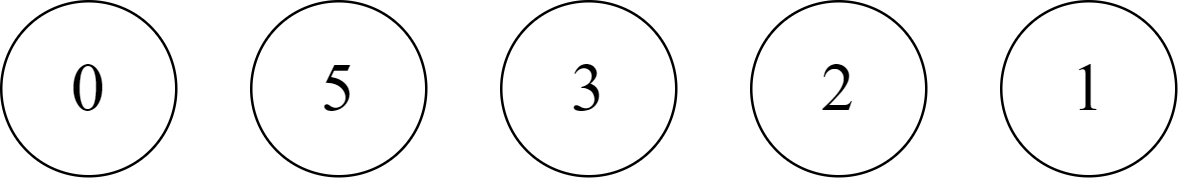
\includegraphics[scale=0.25]{holes1.png}
\end{center}
On their turn, Sammy must pick a hole and eat exactly one acorn from it. Suppose
they pick the third hole. Then the counts become the following:
\begin{center}
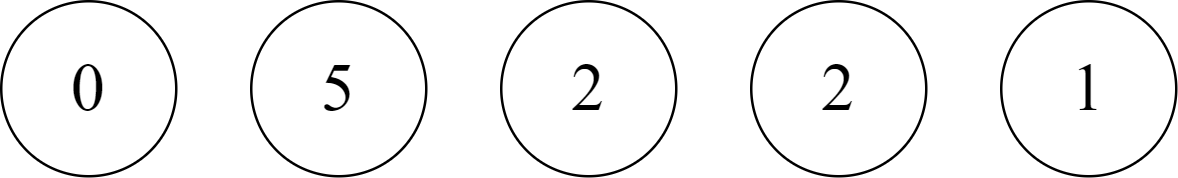
\includegraphics[scale=0.25]{holes2.png}
\end{center}
Sammy may then place any number of extra acorns into each hole to the right of that
hole. In this case, they can place into the fourth and fifth holes. Suppose they
choose to place 3 acorns in the fourth hole and 1 in the fifth. Then the at the end
of Sammy's turn the acorn counts are the following:
\begin{center}
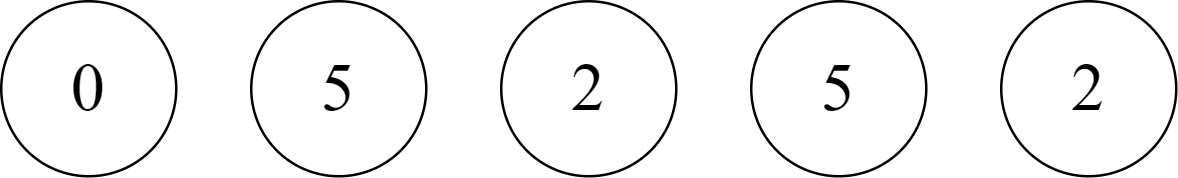
\includegraphics[scale=0.25]{holes3.png}
\end{center}
A winning strategy for a player is a sequence of moves which guarantees that
they will win regardless of what moves their opponent makes. We will construct
a winning strategy for Sammy. We will need an important but non-obvious fact
about this game: the game must reach a state where every hole is
empty except for the right-most hole.
\begin{qparts}
\item Prove that, once we reach the state where all but the right-most hole is
empty,
Sammy has a winning strategy if and only if there are an odd number of acorns
in the hole at the start of their turn.
\item Prove that if a squirrel starts their turn with all holes having an even
number
of acorns (and the game is not over), then at the end of their turn,
at least one hole will have an odd number of acorns.
\item Prove that if a squirrel starts their turn with at least one hole having
an odd number of acorns,
they can end their turn with all holes having an even number of acorns
\item Using the previous parts, prove that Sammy has a winning strategy.
\end{qparts}
\begin{solution}
\begin{qparts}
    \item 
    Let n be an arbitrary integer. There exists n holes.

Case 1: n is odd (there are an odd number of holes)
So there exists an int k such that n = 2k+1.

After turn k:
Sammy will have taken k acorns.
Saph will have taken k acorns.
There will be 2k + 1 - k - k acorns left.
So there will be 1 acorn left.

At turn k+1:
Sammy goes first and eats 1 acorn and ends her turn.
1-1 = 0 acorns left.
Since Saph starts her turn with no acorns, Saph loses and Sammy wins.

Case 2: n is even (there are an even number of holes)
So there exists an int k such that n = 2k.

After turn k:
Sammy will have taken k acorns.
Saph will have taken k acorns.
There will be 2k - k - k acorns left.
So there will be 0 acorns left.

At turn k+1:
Sammy goes first, but there are no acorns left. Sammy loses and Saph wins.

Therefore, Sammy wins if and only if there are an odd \# of acorns at the start of her turn.

\item 
Assume all holes have an even \# of acorns.

So 2a 2b … 2c, $2a + 2b + 2c = 2(a+b+c)$
Because $a,b, c$ are ints,$ a+b+c$ is an int. So the total number of acorns is also even.

Let Sammy take 1 acorn from any hole:
$2(a+b+c) - 1$.
This makes the total number of acorns odd.

Sammy can end her turn without placing any extra acorns, and she will end the turn with at least one hole of odd \# acorns (i.e., the hole that she ate out of). We can prove this statement with a proof by cases: 

If the total number of acorns is odd, then at least one hold is odd.
\begin{enumerate}
    \item Case 1: One hold is odd (then statement proved)
    \item Case 2: No holes are odd. Equivalent to all holes are even. Then total number of acorns will be even: $2(a+b+c…d)$.\\
    This contradicts the assumption
\end{enumerate}

\item 
Assume there is at least one hole with an odd \# of acorns.\\
Let Sammy select the leftmost hole that contains an odd \# of acorns.\\
2n+ 1 2o+1 2p+1 … 2r+1\\
Sammy chooses 2n+1 hole.

Sammy eats one acorn from that hole, making it even.\\ 
then $2(n), 2o+1, 2p+1,\cdots,2r+1$

Sammy can then place 1 acorn into each of the other odd holes, also making them even. \\
then $2(n), 2o+2, 2p+2, … ,2r+2$\\
$2(n), 2(o+1), 2(p+1), … ,2(r+1)$
\\Because Sammy started at the leftmost hole, all odd holes will be accounted for. \\
Thus Sammy always has a way to end the turn with all holes having an even number.

\item  
Given: n holes with 203 holes each.\\
WLOG (regardless if n is odd or even):\\
From c, we know that if Sammy starts w/ at least one odd hole, they can end their turn with all holes having an even \# of acorns. Because all n holes have 203 acorns, there will always be at least one odd hole.\\
Therefore, Sammy can eat an acorn and end her turn in such a way that there will always be all holes with an even \# of acorns.\\
So Sapphire will always start her turn with an even number of acorns.\\
From b, we know that Sapphire has to end her turn with at least one hole having an odd number of acorns.\\
We are given that the game must reach a state where every hole is empty except for the right-most hole.\\
Therefore, the above logic can repeat until there is only one acorn in the right-most hole.\\
Following the logic from part b, since there is an odd number of acorns (i.e., 1), it must be Sammy’s turn.\\
On this turn, Sammy will eat the last acorn and end her turn. 
On Sapphire’s turn, there are no acorns so she loses the game.
\\So in all possible scenarios, Sammy has a winning strategy.
\end{qparts}
\end{solution}
\subsection*{\probnum The Third Dimension [30 Points]}
In lecture, we discussed the problem of tiling a chessboard with dominoes of
dimension $2 \times 1$. We also saw that this question can be made more interesting
by changing the shape of the board.
A related idea to tiling is packing. In a packing question, we no longer care that
the board gets completely covered, instead it is enough to show that a certain
number of dominoes can fit on the board. For example, 32 or fewer $1 \times 2$
dominoes can be packed into a $8 \times 8$ chess board, but 33 or more cannot.
In this problem, we will investigate packing dominoes into a three dimensional
``chess board". In particular, we will prove that it is impossible to pack 53 $1\times 1\times 4$ dominoes into a $6\times 6\times 6$ board.
\begin{qparts}
\item As a warm-up, first show that you \textit{can} pack 54 dominoes into the
board provided that you're allowed to break the dominoes in half.
\item We can divide our board evenly into $2\times 2\times 2$ regions. Consider
coloring these regions red and blue in an alternating fashion. We say that each
$1 \times 1 \times 1$ cell of a domino is colored red if it lies in a red region
and colored blue if it lies in a blue region.
For any domino, list all possible colorings of its 4 cells. Conclude that
exactly half of each domino must lie in a red region.
\item Prove that it is impossible to pack 53 dominoes into a $6\times 6\times
6$ board.
\textbf{Hint:} Figure out how many cells of each color there are, and apply
part (b).
\end{qparts}
\begin{solution}
\begin{qparts}
    \item 
    \begin{center}
        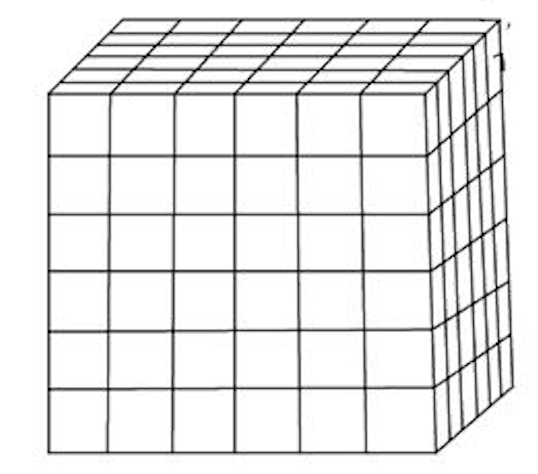
\includegraphics[scale=0.35]{Screenshot 2023-09-28 at 14.26.34.png}
    \end{center}
    
    \begin{center}
        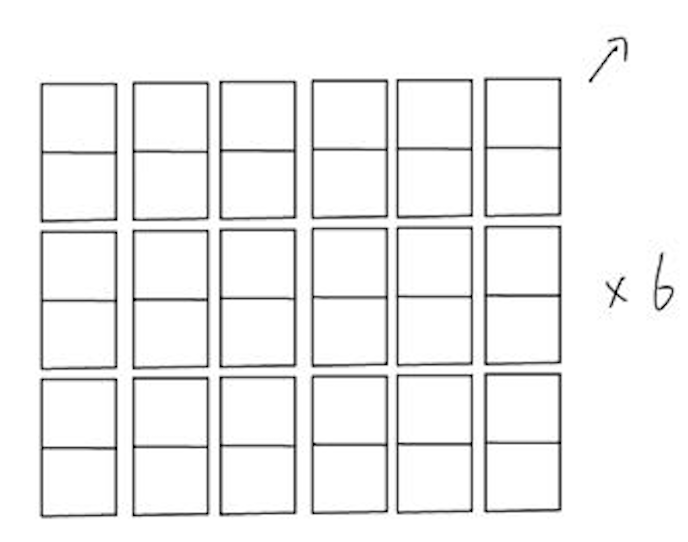
\includegraphics[scale=0.4]{Screenshot 2023-09-28 at 14.26.50.png} 
    \end{center}
    By slicing the cube into 6 identical slices vertically, we have every slice like the picture above. And as we can see, we can fill a slice with $6 \times 3 = 18$ half-dominoes in a slice, and then we fill the 6 identical slices with $18 * 6 = 108$ half-dominoes.
    
    \item 
    \begin{center}
        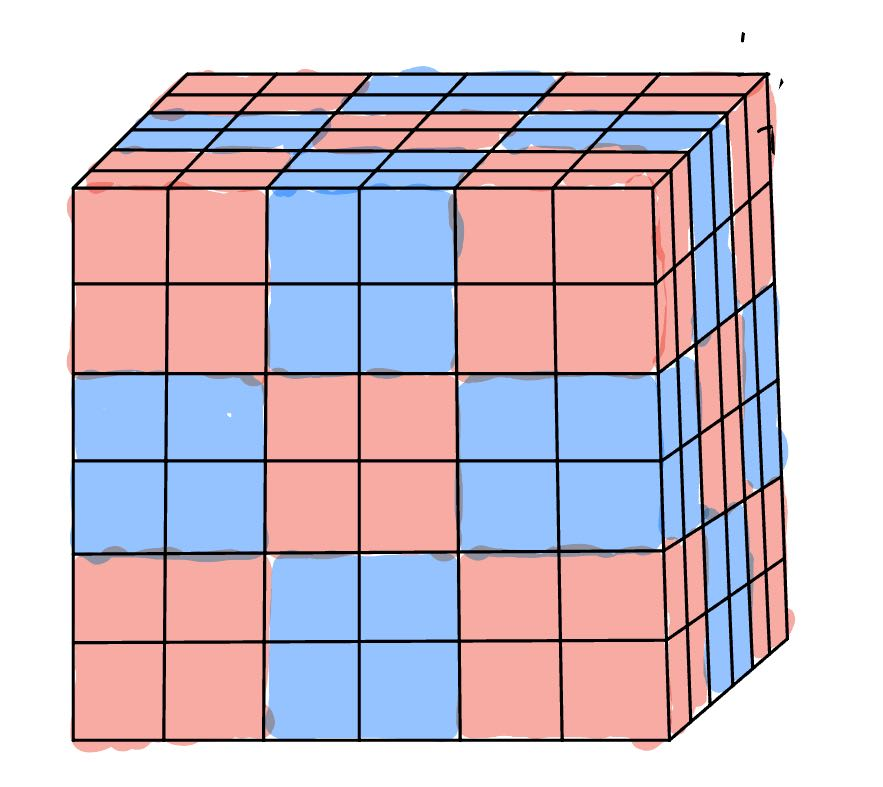
\includegraphics[scale=0.2]{WechatIMG616.jpeg}
    \end{center}
    \begin{center}
        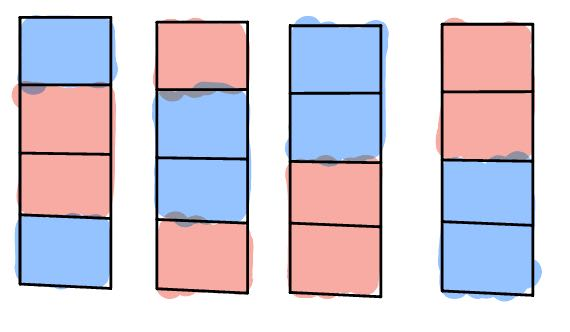
\includegraphics[scale=0.3]{WechatIMG614.jpeg}
    \end{center}
    After we divide the board into $2\times 2\times 2$ regions, if we pack dominoes into the cube board, the 4 possible colorings are as above. We can represent them as BBRR, RRBB, BRRB, RBBR. \\Since every domino contains 2B and 2R, exactly half of each domino must lie in a red region.

    \item 
    After we divide our board into $2 \times 2 \times 2$ regions in alternating color, there should be 27 regions, consisting of 13 blue regions and 14 regions, or 14 blue regions and 13 red regions, dependent on the way we divide.\\
    Since every region contains 8 cells, there would be 8 more blue cells than red cells, or 8 more red cells than blue cells.\\
    Assume that we can pack 53 $1 \times 1 \times 1$ dominoes into the board, then we have $53 \times 2 = 106$ red cells and $53 \times 2 = 106$ blue cells as well.\\
    Then there are $216 - 106 \times 2 = 4$ cells left on the board. Even if they are all red or all blue, that does not meet the quantity. That causes a contradiction.\\
    Therefore we have proved it.
    
\end{qparts}
\end{solution}

\end{document}
